\documentclass[12pt]{article}
\usepackage{fullpage,graphicx,float,psfrag,amsmath,amsfonts}
\usepackage[small,bf]{caption}
\usepackage[numbers,sort&compress]{natbib}
\usepackage[table]{xcolor}
\usepackage{color}
\usepackage{tikz}
\usepackage{verbatim}
\usepackage{minted}
\usepackage{gnuplot-lua-tikz}

\title{
    
\includegraphics[width=0.5in]{images/logo.jpeg}
    CS207 Project: Milestone 1\\
    \large\texttt{@Software-Samurais}
    }
\author{
    Kailas Amin\\ \texttt{kailasamin@college.harvard.edu}
    \and Jingyuan Liu\\ \texttt{jingyuanliu@g.harvard.edu}
    \and Erick Ruiz\\ \texttt{\qquad eruiz@g.harvard.edu  \qquad}
    \and \qquad Simon (Xin) Dong\\ \texttt{\qquad xindong@g.harvard.edu}
    }
\date{October 29, 2019}

\begin{document}

\maketitle

\section{Introduction}
The increasing importance of computational models in science and business alongside the slowing pace of advances in computing hardware has increased the need for efficient and accurate evaluations of derivatives. Many important applications such as simulation, optimization, and neural networks rely on repeated differentiation of complex functions. 

Before the advent of automatic differentiation (AD) the primary method for derivative evaluation was the method of finite differences (FD), where the function to be evaluated is effectively treated as black box oracle.\footnote{See the \emph{Background} section for a more detailed introduction} As the FD method is effectively sampling, the granularity (i.e. step size) of the algorithm can introduce error effects if it is either too large or too small, but even at the perfect medium, $f'(x)$ evaluations cannot reach machine precision. The alternative approach, fully symbolic differentiation (SD), is cumbersome and inefficient in many cases. In the case of a complex computer program, the size of the symbolic expression could grow to outrageous size and cause significant inefficiency.  

The approach of algorithmic differentiation seeks to find the best of both worlds, with machine precision and easy evaluation. This is done by repeated evaluation of the chain rule at a point stored in a table called the computational trace. Thus rather than storing to full symbolic expression, an AD code only needs to apply the chain rule to a specific evaluation, representable by a single variable. This approach allows us to achieve the accuracy of symbolic approaches while drastically reducing the cost of evaluation. 

Within the umbrella of automatic differentiation, we seek to implement the forward mode which evaluates the intermediate results directly in an inside out manner. Other approaches such as reverse mode also have specific advantages especially in the fields of machine learning and artificial intelligence-- or in any context in which the number of inputs dominates the number of outputs.  

The method of automatic differentiation, sometimes also referred to as 
algorithmic differentiation, addresses the weaknesses of the finite 
difference method by providing a systematic way to calculate derivatives 
numerically to arbitrary precision. The goal of \texttt{AutoDiff} is to 
implement the forward mode of automatic differentiation, as it is a relevant
feature that even some mainstream machine learning libraries, such as 
PyTorch, lack. 


\section{Background}
Understanding the concept of a derivative is crucial to all aspiring and 
practicing scientists, engineers, and mathematicians. It is one of the first
concepts introduced in first-year calculus courses at all universities. The 
idea is simple. Given a function, $f(x)$, how can we quantify the rate of 
change of the function due to an infinitesimal change, $\Delta x$, in the 
argument, $x$? The answer is typically given in terms of the limit 
definition of the derivative.
\begin{equation}
    f'(x) = \lim_{\Delta x\rightarrow 0} \frac{f(x+\Delta x)-f(x)}{\Delta x}
    \label{eq:lim-def}
\end{equation}
While equation \eqref{eq:lim-def} holds for any function, in practice, it is
easier to calculate derivatives analytically according to a set of rules. 
However, obtaining an analytical expression for the derivative becomes 
exceedingly difficult if the function of interest is composed of many 
elementary functions. For example, consider the following function.
\begin{equation}
    f(x) = \exp\left[\frac{\sqrt{x^3 - \ln x + \sin(4x^2)}}{\cos(3x^5)}\right]
    \label{eq:ugly-eq}
\end{equation}
Calculating the first derivative would result in the following expression.
\begin{align}
    f'(x) &= \exp\left[\frac{\sqrt{x^3 - \ln x + \sin(4x^2)}}{\cos(3x^5)}\right]
    \sec^2(3x^5)\dots\nonumber\\
    &\qquad\times\left\{
    \frac{\cos(3x^5)}{2\sqrt{x^3 - \ln x + \sin(4x^2)}}
    \left[3x^2-\frac{1}{x}+8x\cos(4x^2)\right]\dots\right.\nonumber\\
    &\qquad\qquad+
    \left.\vphantom{\frac{\cos(3x^5)}{2\sqrt{x^3 - \ln x + \sin(4x^2)}}}
    15x^4\sin(3x^5)\sqrt{x^3 - \ln x + \sin(4x^2)}
    \right\}
\end{align}
Although feasible, successive calculations become more and more complex, and
in practice, the quantity to be differentiated may not be a function in 
closed-form but rather a set of measurements or values given as a 
one-dimensional vector of numbers. In that case, equation \eqref{eq:lim-def}
can be approximated using the finite difference method, which replaces an 
infinitesimal change in the argument for a finite change. To show how this 
works, let us write the Taylor series expansion of an arbitrary function, 
$f(x)$, at the point $x+h$.
\begin{equation}
    f(x+h) = f(x) + hf'(x) + \frac{h^2}{2}f''(x) + \dots
    \label{eq:f-tay}
\end{equation}
Keeping only terms of $\mathcal{O}(h)$ leaves us with
\begin{equation}
    f(x) \approx f(h) + hf'(x),
\end{equation}
which we can rearrange to write an approximate expression for the derivative,
$f'(x)$.
\begin{equation}
    f'(x) \approx \frac{f(x+h)-f(x)}{h}
    \label{eq:fd}
\end{equation}
The finite change, $h$, is called the step size, and equation \eqref{eq:fd} 
is known as the forward difference. Its geometric interpretation is 
described in Figure \ref{fig:fd-schematic}.
\begin{figure}[H]
    \centering
    \begin{tikzpicture}
        % Help lines
        % \draw[help lines] (0,0) grid (6,4);
        
        % Axes
        \draw[<->, >=stealth, thick] (0,4) node[above]{$y$} -- (0,0) -- 
        (6,0) node[right]{$x$};
        
        % Some function
        \draw[smooth, samples=100, domain=0.0:4.85] 
            plot(\x,{0.1*\x^2-1.1*sin(\x)*\x^3+exp(0.1*\x)*\x});
            
        % Tangent line
        \draw[red] (3,3.4) -- (4,2.65);
        
        % Step size
        \draw[dashed] (3,0) -- (3,3.4);
        \draw[dashed] (4,0) -- (4,2.65);
        \draw[|<->|, >=stealth] (3,-0.3) -- (3.5,-0.3) node[fill=white]{$h$}
            -- (4,-0.3);
        
        % Function annotations
        \draw[dashed] (3,3.4) -- (0,3.4) node[left]{$f(x)$};
        \draw[dashed] (4,2.65) -- (0,2.65) node[left]{$f(x+h)$};
    \end{tikzpicture}
    \caption{\textbf{Geometric interpretation of the finite difference 
    method.} As the step size, $h$, decreases, so does the difference 
    between $f(x+h)$ and $f(x)$. In principle, this should lead to a more 
    accurate approximation to the true derivative, $f'(x)$. However, this is
    not always the case.}
    \label{fig:fd-schematic}
\end{figure}

Although the finite difference method is useful and easy to implement, its 
accuracy can vary depending on the step size that is chosen. Suppose we wish
to approximate the derivative of $f(x)=\ln x$ using the forward difference 
method described in equation \eqref{eq:fd} using step sizes $h=\{10^{-1},\,
10^{-7},\,10^{-15}\}$. This is rather unnecessary because the analytical 
derivative is just $f'(x) = 1/x$, but this example will serve to illustrate 
the drawbacks of the finite difference method. At $h=10^{-1}$, the numerical
derivative is inaccurate because the step size is too large, making the 
calculations susceptible to truncation error. Conversely, at $h=10^{-15}$, 
the forward difference method also gives inaccurate results because the 
calculations can only be represented to a finite precision by the hardware 
in use. Hence, rounding error also affects the stability of the finite 
difference method. Figure \ref{fig:fd-accuracy} summarizes the results.
% Finite difference accuracy
% --------------------------
% Borrowed from CS 207: Homework 4, Problem 1 
\begin{figure}[H]
    \centering
    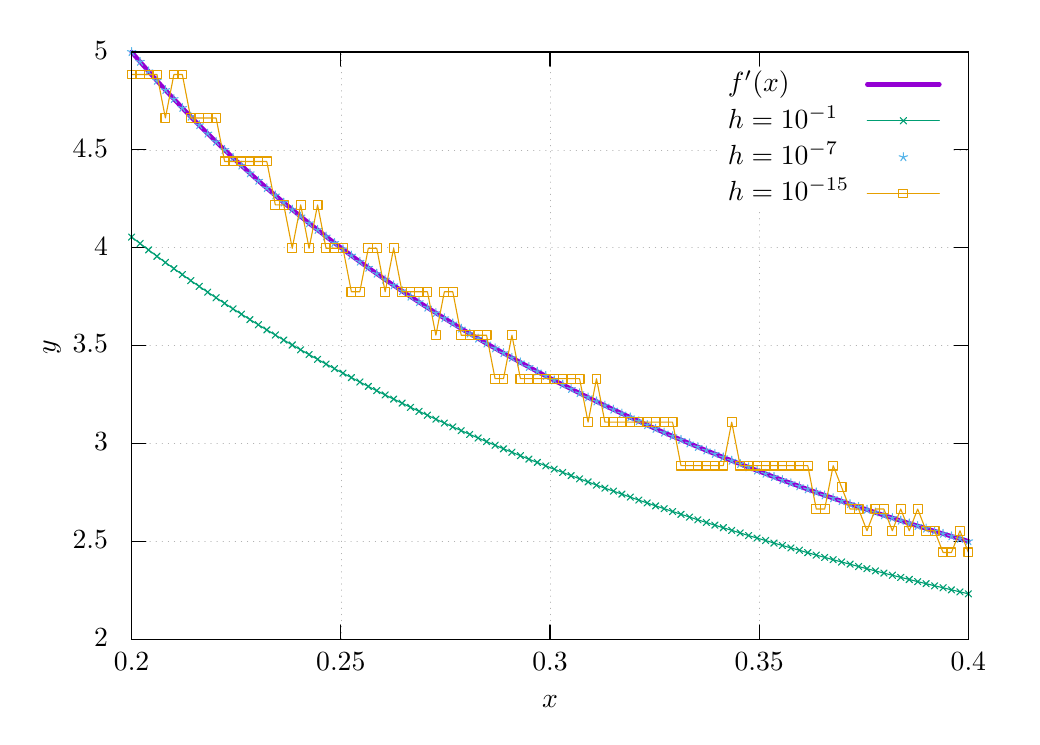
\begin{tikzpicture}[gnuplot]
%% generated with GNUPLOT 5.2p6 (Lua 5.3; terminal rev. Nov 2018, script rev. 107)
%% Sun 27 Oct 2019 07:13:26 PM EDT
\path (0.000,0.000) rectangle (12.500,8.750);
\gpcolor{color=gp lt color axes}
\gpsetlinetype{gp lt axes}
\gpsetdashtype{gp dt axes}
\gpsetlinewidth{0.50}
\draw[gp path] (1.320,0.985)--(11.947,0.985);
\gpcolor{color=gp lt color border}
\gpsetlinetype{gp lt border}
\gpsetdashtype{gp dt solid}
\gpsetlinewidth{1.00}
\draw[gp path] (1.320,0.985)--(1.500,0.985);
\draw[gp path] (11.947,0.985)--(11.767,0.985);
\node[gp node right] at (1.136,0.985) {$2$};
\gpcolor{color=gp lt color axes}
\gpsetlinetype{gp lt axes}
\gpsetdashtype{gp dt axes}
\gpsetlinewidth{0.50}
\draw[gp path] (1.320,2.228)--(11.947,2.228);
\gpcolor{color=gp lt color border}
\gpsetlinetype{gp lt border}
\gpsetdashtype{gp dt solid}
\gpsetlinewidth{1.00}
\draw[gp path] (1.320,2.228)--(1.500,2.228);
\draw[gp path] (11.947,2.228)--(11.767,2.228);
\node[gp node right] at (1.136,2.228) {$2.5$};
\gpcolor{color=gp lt color axes}
\gpsetlinetype{gp lt axes}
\gpsetdashtype{gp dt axes}
\gpsetlinewidth{0.50}
\draw[gp path] (1.320,3.470)--(11.947,3.470);
\gpcolor{color=gp lt color border}
\gpsetlinetype{gp lt border}
\gpsetdashtype{gp dt solid}
\gpsetlinewidth{1.00}
\draw[gp path] (1.320,3.470)--(1.500,3.470);
\draw[gp path] (11.947,3.470)--(11.767,3.470);
\node[gp node right] at (1.136,3.470) {$3$};
\gpcolor{color=gp lt color axes}
\gpsetlinetype{gp lt axes}
\gpsetdashtype{gp dt axes}
\gpsetlinewidth{0.50}
\draw[gp path] (1.320,4.713)--(11.947,4.713);
\gpcolor{color=gp lt color border}
\gpsetlinetype{gp lt border}
\gpsetdashtype{gp dt solid}
\gpsetlinewidth{1.00}
\draw[gp path] (1.320,4.713)--(1.500,4.713);
\draw[gp path] (11.947,4.713)--(11.767,4.713);
\node[gp node right] at (1.136,4.713) {$3.5$};
\gpcolor{color=gp lt color axes}
\gpsetlinetype{gp lt axes}
\gpsetdashtype{gp dt axes}
\gpsetlinewidth{0.50}
\draw[gp path] (1.320,5.956)--(11.947,5.956);
\gpcolor{color=gp lt color border}
\gpsetlinetype{gp lt border}
\gpsetdashtype{gp dt solid}
\gpsetlinewidth{1.00}
\draw[gp path] (1.320,5.956)--(1.500,5.956);
\draw[gp path] (11.947,5.956)--(11.767,5.956);
\node[gp node right] at (1.136,5.956) {$4$};
\gpcolor{color=gp lt color axes}
\gpsetlinetype{gp lt axes}
\gpsetdashtype{gp dt axes}
\gpsetlinewidth{0.50}
\draw[gp path] (1.320,7.198)--(8.777,7.198);
\draw[gp path] (11.763,7.198)--(11.947,7.198);
\gpcolor{color=gp lt color border}
\gpsetlinetype{gp lt border}
\gpsetdashtype{gp dt solid}
\gpsetlinewidth{1.00}
\draw[gp path] (1.320,7.198)--(1.500,7.198);
\draw[gp path] (11.947,7.198)--(11.767,7.198);
\node[gp node right] at (1.136,7.198) {$4.5$};
\gpcolor{color=gp lt color axes}
\gpsetlinetype{gp lt axes}
\gpsetdashtype{gp dt axes}
\gpsetlinewidth{0.50}
\draw[gp path] (1.320,8.441)--(11.947,8.441);
\gpcolor{color=gp lt color border}
\gpsetlinetype{gp lt border}
\gpsetdashtype{gp dt solid}
\gpsetlinewidth{1.00}
\draw[gp path] (1.320,8.441)--(1.500,8.441);
\draw[gp path] (11.947,8.441)--(11.767,8.441);
\node[gp node right] at (1.136,8.441) {$5$};
\gpcolor{color=gp lt color axes}
\gpsetlinetype{gp lt axes}
\gpsetdashtype{gp dt axes}
\gpsetlinewidth{0.50}
\draw[gp path] (1.320,0.985)--(1.320,8.441);
\gpcolor{color=gp lt color border}
\gpsetlinetype{gp lt border}
\gpsetdashtype{gp dt solid}
\gpsetlinewidth{1.00}
\draw[gp path] (1.320,0.985)--(1.320,1.165);
\draw[gp path] (1.320,8.441)--(1.320,8.261);
\node[gp node center] at (1.320,0.677) {$0.2$};
\gpcolor{color=gp lt color axes}
\gpsetlinetype{gp lt axes}
\gpsetdashtype{gp dt axes}
\gpsetlinewidth{0.50}
\draw[gp path] (3.977,0.985)--(3.977,8.441);
\gpcolor{color=gp lt color border}
\gpsetlinetype{gp lt border}
\gpsetdashtype{gp dt solid}
\gpsetlinewidth{1.00}
\draw[gp path] (3.977,0.985)--(3.977,1.165);
\draw[gp path] (3.977,8.441)--(3.977,8.261);
\node[gp node center] at (3.977,0.677) {$0.25$};
\gpcolor{color=gp lt color axes}
\gpsetlinetype{gp lt axes}
\gpsetdashtype{gp dt axes}
\gpsetlinewidth{0.50}
\draw[gp path] (6.633,0.985)--(6.633,8.441);
\gpcolor{color=gp lt color border}
\gpsetlinetype{gp lt border}
\gpsetdashtype{gp dt solid}
\gpsetlinewidth{1.00}
\draw[gp path] (6.633,0.985)--(6.633,1.165);
\draw[gp path] (6.633,8.441)--(6.633,8.261);
\node[gp node center] at (6.633,0.677) {$0.3$};
\gpcolor{color=gp lt color axes}
\gpsetlinetype{gp lt axes}
\gpsetdashtype{gp dt axes}
\gpsetlinewidth{0.50}
\draw[gp path] (9.290,0.985)--(9.290,6.413);
\draw[gp path] (9.290,8.261)--(9.290,8.441);
\gpcolor{color=gp lt color border}
\gpsetlinetype{gp lt border}
\gpsetdashtype{gp dt solid}
\gpsetlinewidth{1.00}
\draw[gp path] (9.290,0.985)--(9.290,1.165);
\draw[gp path] (9.290,8.441)--(9.290,8.261);
\node[gp node center] at (9.290,0.677) {$0.35$};
\gpcolor{color=gp lt color axes}
\gpsetlinetype{gp lt axes}
\gpsetdashtype{gp dt axes}
\gpsetlinewidth{0.50}
\draw[gp path] (11.947,0.985)--(11.947,8.441);
\gpcolor{color=gp lt color border}
\gpsetlinetype{gp lt border}
\gpsetdashtype{gp dt solid}
\gpsetlinewidth{1.00}
\draw[gp path] (11.947,0.985)--(11.947,1.165);
\draw[gp path] (11.947,8.441)--(11.947,8.261);
\node[gp node center] at (11.947,0.677) {$0.4$};
\draw[gp path] (1.320,8.441)--(1.320,0.985)--(11.947,0.985)--(11.947,8.441)--cycle;
\node[gp node center,rotate=-270] at (0.276,4.713) {$y$};
\node[gp node center] at (6.633,0.215) {$x$};
\node[gp node left] at (8.777,8.030) {$f'(x)$};
\gpcolor{rgb color={0.580,0.000,0.827}}
\gpsetlinewidth{4.00}
\draw[gp path] (10.663,8.030)--(11.579,8.030);
\draw[gp path] (1.320,8.441)--(1.427,8.317)--(1.535,8.195)--(1.642,8.076)--(1.749,7.958)%
  --(1.857,7.844)--(1.964,7.731)--(2.071,7.620)--(2.179,7.512)--(2.286,7.405)--(2.393,7.301)%
  --(2.501,7.198)--(2.608,7.098)--(2.715,6.999)--(2.823,6.901)--(2.930,6.806)--(3.037,6.712)%
  --(3.145,6.620)--(3.252,6.529)--(3.360,6.440)--(3.467,6.352)--(3.574,6.266)--(3.682,6.182)%
  --(3.789,6.098)--(3.896,6.016)--(4.004,5.936)--(4.111,5.856)--(4.218,5.778)--(4.326,5.701)%
  --(4.433,5.626)--(4.540,5.551)--(4.648,5.478)--(4.755,5.405)--(4.862,5.334)--(4.970,5.264)%
  --(5.077,5.195)--(5.184,5.127)--(5.292,5.060)--(5.399,4.994)--(5.506,4.929)--(5.614,4.865)%
  --(5.721,4.802)--(5.828,4.739)--(5.936,4.678)--(6.043,4.617)--(6.150,4.558)--(6.258,4.499)%
  --(6.365,4.441)--(6.472,4.383)--(6.580,4.327)--(6.687,4.271)--(6.795,4.216)--(6.902,4.162)%
  --(7.009,4.108)--(7.117,4.055)--(7.224,4.003)--(7.331,3.951)--(7.439,3.900)--(7.546,3.850)%
  --(7.653,3.801)--(7.761,3.752)--(7.868,3.703)--(7.975,3.656)--(8.083,3.608)--(8.190,3.562)%
  --(8.297,3.516)--(8.405,3.470)--(8.512,3.425)--(8.619,3.381)--(8.727,3.337)--(8.834,3.294)%
  --(8.941,3.251)--(9.049,3.209)--(9.156,3.167)--(9.263,3.126)--(9.371,3.085)--(9.478,3.044)%
  --(9.585,3.004)--(9.693,2.965)--(9.800,2.926)--(9.907,2.887)--(10.015,2.849)--(10.122,2.811)%
  --(10.230,2.774)--(10.337,2.737)--(10.444,2.700)--(10.552,2.664)--(10.659,2.629)--(10.766,2.593)%
  --(10.874,2.558)--(10.981,2.524)--(11.088,2.489)--(11.196,2.455)--(11.303,2.422)--(11.410,2.389)%
  --(11.518,2.356)--(11.625,2.323)--(11.732,2.291)--(11.840,2.259)--(11.947,2.228);
\gpcolor{color=gp lt color border}
\node[gp node left] at (8.777,7.568) {$h=10^{-1}$};
\gpcolor{rgb color={0.000,0.620,0.451}}
\gpsetlinewidth{1.00}
\draw[gp path] (10.663,7.568)--(11.579,7.568);
\draw[gp path] (1.320,6.091)--(1.427,6.009)--(1.535,5.927)--(1.642,5.847)--(1.749,5.768)%
  --(1.857,5.690)--(1.964,5.614)--(2.071,5.538)--(2.179,5.464)--(2.286,5.391)--(2.393,5.320)%
  --(2.501,5.249)--(2.608,5.179)--(2.715,5.111)--(2.823,5.043)--(2.930,4.977)--(3.037,4.911)%
  --(3.145,4.847)--(3.252,4.783)--(3.360,4.720)--(3.467,4.659)--(3.574,4.598)--(3.682,4.538)%
  --(3.789,4.478)--(3.896,4.420)--(4.004,4.362)--(4.111,4.306)--(4.218,4.250)--(4.326,4.194)%
  --(4.433,4.140)--(4.540,4.086)--(4.648,4.033)--(4.755,3.981)--(4.862,3.929)--(4.970,3.878)%
  --(5.077,3.828)--(5.184,3.778)--(5.292,3.729)--(5.399,3.680)--(5.506,3.633)--(5.614,3.585)%
  --(5.721,3.539)--(5.828,3.493)--(5.936,3.447)--(6.043,3.402)--(6.150,3.358)--(6.258,3.314)%
  --(6.365,3.270)--(6.472,3.228)--(6.580,3.185)--(6.687,3.143)--(6.795,3.102)--(6.902,3.061)%
  --(7.009,3.021)--(7.117,2.981)--(7.224,2.941)--(7.331,2.902)--(7.439,2.864)--(7.546,2.826)%
  --(7.653,2.788)--(7.761,2.750)--(7.868,2.714)--(7.975,2.677)--(8.083,2.641)--(8.190,2.605)%
  --(8.297,2.570)--(8.405,2.535)--(8.512,2.500)--(8.619,2.466)--(8.727,2.432)--(8.834,2.399)%
  --(8.941,2.366)--(9.049,2.333)--(9.156,2.300)--(9.263,2.268)--(9.371,2.237)--(9.478,2.205)%
  --(9.585,2.174)--(9.693,2.143)--(9.800,2.113)--(9.907,2.082)--(10.015,2.052)--(10.122,2.023)%
  --(10.230,1.993)--(10.337,1.964)--(10.444,1.936)--(10.552,1.907)--(10.659,1.879)--(10.766,1.851)%
  --(10.874,1.823)--(10.981,1.796)--(11.088,1.769)--(11.196,1.742)--(11.303,1.715)--(11.410,1.689)%
  --(11.518,1.662)--(11.625,1.637)--(11.732,1.611)--(11.840,1.585)--(11.947,1.560);
\gpsetpointsize{4.00}
\gppoint{gp mark 2}{(1.320,6.091)}
\gppoint{gp mark 2}{(1.427,6.009)}
\gppoint{gp mark 2}{(1.535,5.927)}
\gppoint{gp mark 2}{(1.642,5.847)}
\gppoint{gp mark 2}{(1.749,5.768)}
\gppoint{gp mark 2}{(1.857,5.690)}
\gppoint{gp mark 2}{(1.964,5.614)}
\gppoint{gp mark 2}{(2.071,5.538)}
\gppoint{gp mark 2}{(2.179,5.464)}
\gppoint{gp mark 2}{(2.286,5.391)}
\gppoint{gp mark 2}{(2.393,5.320)}
\gppoint{gp mark 2}{(2.501,5.249)}
\gppoint{gp mark 2}{(2.608,5.179)}
\gppoint{gp mark 2}{(2.715,5.111)}
\gppoint{gp mark 2}{(2.823,5.043)}
\gppoint{gp mark 2}{(2.930,4.977)}
\gppoint{gp mark 2}{(3.037,4.911)}
\gppoint{gp mark 2}{(3.145,4.847)}
\gppoint{gp mark 2}{(3.252,4.783)}
\gppoint{gp mark 2}{(3.360,4.720)}
\gppoint{gp mark 2}{(3.467,4.659)}
\gppoint{gp mark 2}{(3.574,4.598)}
\gppoint{gp mark 2}{(3.682,4.538)}
\gppoint{gp mark 2}{(3.789,4.478)}
\gppoint{gp mark 2}{(3.896,4.420)}
\gppoint{gp mark 2}{(4.004,4.362)}
\gppoint{gp mark 2}{(4.111,4.306)}
\gppoint{gp mark 2}{(4.218,4.250)}
\gppoint{gp mark 2}{(4.326,4.194)}
\gppoint{gp mark 2}{(4.433,4.140)}
\gppoint{gp mark 2}{(4.540,4.086)}
\gppoint{gp mark 2}{(4.648,4.033)}
\gppoint{gp mark 2}{(4.755,3.981)}
\gppoint{gp mark 2}{(4.862,3.929)}
\gppoint{gp mark 2}{(4.970,3.878)}
\gppoint{gp mark 2}{(5.077,3.828)}
\gppoint{gp mark 2}{(5.184,3.778)}
\gppoint{gp mark 2}{(5.292,3.729)}
\gppoint{gp mark 2}{(5.399,3.680)}
\gppoint{gp mark 2}{(5.506,3.633)}
\gppoint{gp mark 2}{(5.614,3.585)}
\gppoint{gp mark 2}{(5.721,3.539)}
\gppoint{gp mark 2}{(5.828,3.493)}
\gppoint{gp mark 2}{(5.936,3.447)}
\gppoint{gp mark 2}{(6.043,3.402)}
\gppoint{gp mark 2}{(6.150,3.358)}
\gppoint{gp mark 2}{(6.258,3.314)}
\gppoint{gp mark 2}{(6.365,3.270)}
\gppoint{gp mark 2}{(6.472,3.228)}
\gppoint{gp mark 2}{(6.580,3.185)}
\gppoint{gp mark 2}{(6.687,3.143)}
\gppoint{gp mark 2}{(6.795,3.102)}
\gppoint{gp mark 2}{(6.902,3.061)}
\gppoint{gp mark 2}{(7.009,3.021)}
\gppoint{gp mark 2}{(7.117,2.981)}
\gppoint{gp mark 2}{(7.224,2.941)}
\gppoint{gp mark 2}{(7.331,2.902)}
\gppoint{gp mark 2}{(7.439,2.864)}
\gppoint{gp mark 2}{(7.546,2.826)}
\gppoint{gp mark 2}{(7.653,2.788)}
\gppoint{gp mark 2}{(7.761,2.750)}
\gppoint{gp mark 2}{(7.868,2.714)}
\gppoint{gp mark 2}{(7.975,2.677)}
\gppoint{gp mark 2}{(8.083,2.641)}
\gppoint{gp mark 2}{(8.190,2.605)}
\gppoint{gp mark 2}{(8.297,2.570)}
\gppoint{gp mark 2}{(8.405,2.535)}
\gppoint{gp mark 2}{(8.512,2.500)}
\gppoint{gp mark 2}{(8.619,2.466)}
\gppoint{gp mark 2}{(8.727,2.432)}
\gppoint{gp mark 2}{(8.834,2.399)}
\gppoint{gp mark 2}{(8.941,2.366)}
\gppoint{gp mark 2}{(9.049,2.333)}
\gppoint{gp mark 2}{(9.156,2.300)}
\gppoint{gp mark 2}{(9.263,2.268)}
\gppoint{gp mark 2}{(9.371,2.237)}
\gppoint{gp mark 2}{(9.478,2.205)}
\gppoint{gp mark 2}{(9.585,2.174)}
\gppoint{gp mark 2}{(9.693,2.143)}
\gppoint{gp mark 2}{(9.800,2.113)}
\gppoint{gp mark 2}{(9.907,2.082)}
\gppoint{gp mark 2}{(10.015,2.052)}
\gppoint{gp mark 2}{(10.122,2.023)}
\gppoint{gp mark 2}{(10.230,1.993)}
\gppoint{gp mark 2}{(10.337,1.964)}
\gppoint{gp mark 2}{(10.444,1.936)}
\gppoint{gp mark 2}{(10.552,1.907)}
\gppoint{gp mark 2}{(10.659,1.879)}
\gppoint{gp mark 2}{(10.766,1.851)}
\gppoint{gp mark 2}{(10.874,1.823)}
\gppoint{gp mark 2}{(10.981,1.796)}
\gppoint{gp mark 2}{(11.088,1.769)}
\gppoint{gp mark 2}{(11.196,1.742)}
\gppoint{gp mark 2}{(11.303,1.715)}
\gppoint{gp mark 2}{(11.410,1.689)}
\gppoint{gp mark 2}{(11.518,1.662)}
\gppoint{gp mark 2}{(11.625,1.637)}
\gppoint{gp mark 2}{(11.732,1.611)}
\gppoint{gp mark 2}{(11.840,1.585)}
\gppoint{gp mark 2}{(11.947,1.560)}
\gppoint{gp mark 2}{(11.121,7.568)}
\gpcolor{color=gp lt color border}
\node[gp node left] at (8.777,7.106) {$h=10^{-7}$};
\gpcolor{rgb color={0.337,0.706,0.914}}
\gppoint{gp mark 3}{(1.320,8.441)}
\gppoint{gp mark 3}{(1.427,8.317)}
\gppoint{gp mark 3}{(1.535,8.195)}
\gppoint{gp mark 3}{(1.642,8.076)}
\gppoint{gp mark 3}{(1.749,7.958)}
\gppoint{gp mark 3}{(1.857,7.844)}
\gppoint{gp mark 3}{(1.964,7.731)}
\gppoint{gp mark 3}{(2.071,7.620)}
\gppoint{gp mark 3}{(2.179,7.512)}
\gppoint{gp mark 3}{(2.286,7.405)}
\gppoint{gp mark 3}{(2.393,7.301)}
\gppoint{gp mark 3}{(2.501,7.198)}
\gppoint{gp mark 3}{(2.608,7.098)}
\gppoint{gp mark 3}{(2.715,6.999)}
\gppoint{gp mark 3}{(2.823,6.901)}
\gppoint{gp mark 3}{(2.930,6.806)}
\gppoint{gp mark 3}{(3.037,6.712)}
\gppoint{gp mark 3}{(3.145,6.620)}
\gppoint{gp mark 3}{(3.252,6.529)}
\gppoint{gp mark 3}{(3.360,6.440)}
\gppoint{gp mark 3}{(3.467,6.352)}
\gppoint{gp mark 3}{(3.574,6.266)}
\gppoint{gp mark 3}{(3.682,6.182)}
\gppoint{gp mark 3}{(3.789,6.098)}
\gppoint{gp mark 3}{(3.896,6.016)}
\gppoint{gp mark 3}{(4.004,5.936)}
\gppoint{gp mark 3}{(4.111,5.856)}
\gppoint{gp mark 3}{(4.218,5.778)}
\gppoint{gp mark 3}{(4.326,5.701)}
\gppoint{gp mark 3}{(4.433,5.626)}
\gppoint{gp mark 3}{(4.540,5.551)}
\gppoint{gp mark 3}{(4.648,5.478)}
\gppoint{gp mark 3}{(4.755,5.405)}
\gppoint{gp mark 3}{(4.862,5.334)}
\gppoint{gp mark 3}{(4.970,5.264)}
\gppoint{gp mark 3}{(5.077,5.195)}
\gppoint{gp mark 3}{(5.184,5.127)}
\gppoint{gp mark 3}{(5.292,5.060)}
\gppoint{gp mark 3}{(5.399,4.994)}
\gppoint{gp mark 3}{(5.506,4.929)}
\gppoint{gp mark 3}{(5.614,4.865)}
\gppoint{gp mark 3}{(5.721,4.802)}
\gppoint{gp mark 3}{(5.828,4.739)}
\gppoint{gp mark 3}{(5.936,4.678)}
\gppoint{gp mark 3}{(6.043,4.617)}
\gppoint{gp mark 3}{(6.150,4.558)}
\gppoint{gp mark 3}{(6.258,4.499)}
\gppoint{gp mark 3}{(6.365,4.441)}
\gppoint{gp mark 3}{(6.472,4.383)}
\gppoint{gp mark 3}{(6.580,4.327)}
\gppoint{gp mark 3}{(6.687,4.271)}
\gppoint{gp mark 3}{(6.795,4.216)}
\gppoint{gp mark 3}{(6.902,4.162)}
\gppoint{gp mark 3}{(7.009,4.108)}
\gppoint{gp mark 3}{(7.117,4.055)}
\gppoint{gp mark 3}{(7.224,4.003)}
\gppoint{gp mark 3}{(7.331,3.951)}
\gppoint{gp mark 3}{(7.439,3.900)}
\gppoint{gp mark 3}{(7.546,3.850)}
\gppoint{gp mark 3}{(7.653,3.801)}
\gppoint{gp mark 3}{(7.761,3.752)}
\gppoint{gp mark 3}{(7.868,3.703)}
\gppoint{gp mark 3}{(7.975,3.656)}
\gppoint{gp mark 3}{(8.083,3.608)}
\gppoint{gp mark 3}{(8.190,3.562)}
\gppoint{gp mark 3}{(8.297,3.516)}
\gppoint{gp mark 3}{(8.405,3.470)}
\gppoint{gp mark 3}{(8.512,3.425)}
\gppoint{gp mark 3}{(8.619,3.381)}
\gppoint{gp mark 3}{(8.727,3.337)}
\gppoint{gp mark 3}{(8.834,3.294)}
\gppoint{gp mark 3}{(8.941,3.251)}
\gppoint{gp mark 3}{(9.049,3.209)}
\gppoint{gp mark 3}{(9.156,3.167)}
\gppoint{gp mark 3}{(9.263,3.126)}
\gppoint{gp mark 3}{(9.371,3.085)}
\gppoint{gp mark 3}{(9.478,3.044)}
\gppoint{gp mark 3}{(9.585,3.004)}
\gppoint{gp mark 3}{(9.693,2.965)}
\gppoint{gp mark 3}{(9.800,2.926)}
\gppoint{gp mark 3}{(9.907,2.887)}
\gppoint{gp mark 3}{(10.015,2.849)}
\gppoint{gp mark 3}{(10.122,2.811)}
\gppoint{gp mark 3}{(10.230,2.774)}
\gppoint{gp mark 3}{(10.337,2.737)}
\gppoint{gp mark 3}{(10.444,2.700)}
\gppoint{gp mark 3}{(10.552,2.664)}
\gppoint{gp mark 3}{(10.659,2.629)}
\gppoint{gp mark 3}{(10.766,2.593)}
\gppoint{gp mark 3}{(10.874,2.558)}
\gppoint{gp mark 3}{(10.981,2.524)}
\gppoint{gp mark 3}{(11.088,2.489)}
\gppoint{gp mark 3}{(11.196,2.455)}
\gppoint{gp mark 3}{(11.303,2.422)}
\gppoint{gp mark 3}{(11.410,2.389)}
\gppoint{gp mark 3}{(11.518,2.356)}
\gppoint{gp mark 3}{(11.625,2.323)}
\gppoint{gp mark 3}{(11.732,2.291)}
\gppoint{gp mark 3}{(11.840,2.259)}
\gppoint{gp mark 3}{(11.947,2.228)}
\gppoint{gp mark 3}{(11.121,7.106)}
\gpcolor{color=gp lt color border}
\node[gp node left] at (8.777,6.644) {$h=10^{-15}$};
\gpcolor{rgb color={0.902,0.624,0.000}}
\draw[gp path] (10.663,6.644)--(11.579,6.644);
\draw[gp path] (1.320,8.155)--(1.427,8.155)--(1.535,8.155)--(1.642,8.155)--(1.749,7.603)%
  --(1.857,8.155)--(1.964,8.155)--(2.071,7.603)--(2.179,7.603)--(2.286,7.603)--(2.393,7.603)%
  --(2.501,7.051)--(2.608,7.051)--(2.715,7.051)--(2.823,7.051)--(2.930,7.051)--(3.037,7.051)%
  --(3.145,6.500)--(3.252,6.500)--(3.360,5.948)--(3.467,6.500)--(3.574,5.948)--(3.682,6.500)%
  --(3.789,5.948)--(3.896,5.948)--(4.004,5.948)--(4.111,5.396)--(4.218,5.396)--(4.326,5.948)%
  --(4.433,5.948)--(4.540,5.396)--(4.648,5.948)--(4.755,5.396)--(4.862,5.396)--(4.970,5.396)%
  --(5.077,5.396)--(5.184,4.844)--(5.292,5.396)--(5.399,5.396)--(5.506,4.844)--(5.614,4.844)%
  --(5.721,4.844)--(5.828,4.844)--(5.936,4.292)--(6.043,4.292)--(6.150,4.844)--(6.258,4.292)%
  --(6.365,4.292)--(6.472,4.292)--(6.580,4.292)--(6.687,4.292)--(6.795,4.292)--(6.902,4.292)%
  --(7.009,4.292)--(7.117,3.740)--(7.224,4.292)--(7.331,3.740)--(7.439,3.740)--(7.546,3.740)%
  --(7.653,3.740)--(7.761,3.740)--(7.868,3.740)--(7.975,3.740)--(8.083,3.740)--(8.190,3.740)%
  --(8.297,3.188)--(8.405,3.188)--(8.512,3.188)--(8.619,3.188)--(8.727,3.188)--(8.834,3.188)%
  --(8.941,3.740)--(9.049,3.188)--(9.156,3.188)--(9.263,3.188)--(9.371,3.188)--(9.478,3.188)%
  --(9.585,3.188)--(9.693,3.188)--(9.800,3.188)--(9.907,3.188)--(10.015,2.637)--(10.122,2.637)%
  --(10.230,3.188)--(10.337,2.913)--(10.444,2.637)--(10.552,2.637)--(10.659,2.361)--(10.766,2.637)%
  --(10.874,2.637)--(10.981,2.361)--(11.088,2.637)--(11.196,2.361)--(11.303,2.637)--(11.410,2.361)%
  --(11.518,2.361)--(11.625,2.085)--(11.732,2.085)--(11.840,2.361)--(11.947,2.085);
\gppoint{gp mark 4}{(1.320,8.155)}
\gppoint{gp mark 4}{(1.427,8.155)}
\gppoint{gp mark 4}{(1.535,8.155)}
\gppoint{gp mark 4}{(1.642,8.155)}
\gppoint{gp mark 4}{(1.749,7.603)}
\gppoint{gp mark 4}{(1.857,8.155)}
\gppoint{gp mark 4}{(1.964,8.155)}
\gppoint{gp mark 4}{(2.071,7.603)}
\gppoint{gp mark 4}{(2.179,7.603)}
\gppoint{gp mark 4}{(2.286,7.603)}
\gppoint{gp mark 4}{(2.393,7.603)}
\gppoint{gp mark 4}{(2.501,7.051)}
\gppoint{gp mark 4}{(2.608,7.051)}
\gppoint{gp mark 4}{(2.715,7.051)}
\gppoint{gp mark 4}{(2.823,7.051)}
\gppoint{gp mark 4}{(2.930,7.051)}
\gppoint{gp mark 4}{(3.037,7.051)}
\gppoint{gp mark 4}{(3.145,6.500)}
\gppoint{gp mark 4}{(3.252,6.500)}
\gppoint{gp mark 4}{(3.360,5.948)}
\gppoint{gp mark 4}{(3.467,6.500)}
\gppoint{gp mark 4}{(3.574,5.948)}
\gppoint{gp mark 4}{(3.682,6.500)}
\gppoint{gp mark 4}{(3.789,5.948)}
\gppoint{gp mark 4}{(3.896,5.948)}
\gppoint{gp mark 4}{(4.004,5.948)}
\gppoint{gp mark 4}{(4.111,5.396)}
\gppoint{gp mark 4}{(4.218,5.396)}
\gppoint{gp mark 4}{(4.326,5.948)}
\gppoint{gp mark 4}{(4.433,5.948)}
\gppoint{gp mark 4}{(4.540,5.396)}
\gppoint{gp mark 4}{(4.648,5.948)}
\gppoint{gp mark 4}{(4.755,5.396)}
\gppoint{gp mark 4}{(4.862,5.396)}
\gppoint{gp mark 4}{(4.970,5.396)}
\gppoint{gp mark 4}{(5.077,5.396)}
\gppoint{gp mark 4}{(5.184,4.844)}
\gppoint{gp mark 4}{(5.292,5.396)}
\gppoint{gp mark 4}{(5.399,5.396)}
\gppoint{gp mark 4}{(5.506,4.844)}
\gppoint{gp mark 4}{(5.614,4.844)}
\gppoint{gp mark 4}{(5.721,4.844)}
\gppoint{gp mark 4}{(5.828,4.844)}
\gppoint{gp mark 4}{(5.936,4.292)}
\gppoint{gp mark 4}{(6.043,4.292)}
\gppoint{gp mark 4}{(6.150,4.844)}
\gppoint{gp mark 4}{(6.258,4.292)}
\gppoint{gp mark 4}{(6.365,4.292)}
\gppoint{gp mark 4}{(6.472,4.292)}
\gppoint{gp mark 4}{(6.580,4.292)}
\gppoint{gp mark 4}{(6.687,4.292)}
\gppoint{gp mark 4}{(6.795,4.292)}
\gppoint{gp mark 4}{(6.902,4.292)}
\gppoint{gp mark 4}{(7.009,4.292)}
\gppoint{gp mark 4}{(7.117,3.740)}
\gppoint{gp mark 4}{(7.224,4.292)}
\gppoint{gp mark 4}{(7.331,3.740)}
\gppoint{gp mark 4}{(7.439,3.740)}
\gppoint{gp mark 4}{(7.546,3.740)}
\gppoint{gp mark 4}{(7.653,3.740)}
\gppoint{gp mark 4}{(7.761,3.740)}
\gppoint{gp mark 4}{(7.868,3.740)}
\gppoint{gp mark 4}{(7.975,3.740)}
\gppoint{gp mark 4}{(8.083,3.740)}
\gppoint{gp mark 4}{(8.190,3.740)}
\gppoint{gp mark 4}{(8.297,3.188)}
\gppoint{gp mark 4}{(8.405,3.188)}
\gppoint{gp mark 4}{(8.512,3.188)}
\gppoint{gp mark 4}{(8.619,3.188)}
\gppoint{gp mark 4}{(8.727,3.188)}
\gppoint{gp mark 4}{(8.834,3.188)}
\gppoint{gp mark 4}{(8.941,3.740)}
\gppoint{gp mark 4}{(9.049,3.188)}
\gppoint{gp mark 4}{(9.156,3.188)}
\gppoint{gp mark 4}{(9.263,3.188)}
\gppoint{gp mark 4}{(9.371,3.188)}
\gppoint{gp mark 4}{(9.478,3.188)}
\gppoint{gp mark 4}{(9.585,3.188)}
\gppoint{gp mark 4}{(9.693,3.188)}
\gppoint{gp mark 4}{(9.800,3.188)}
\gppoint{gp mark 4}{(9.907,3.188)}
\gppoint{gp mark 4}{(10.015,2.637)}
\gppoint{gp mark 4}{(10.122,2.637)}
\gppoint{gp mark 4}{(10.230,3.188)}
\gppoint{gp mark 4}{(10.337,2.913)}
\gppoint{gp mark 4}{(10.444,2.637)}
\gppoint{gp mark 4}{(10.552,2.637)}
\gppoint{gp mark 4}{(10.659,2.361)}
\gppoint{gp mark 4}{(10.766,2.637)}
\gppoint{gp mark 4}{(10.874,2.637)}
\gppoint{gp mark 4}{(10.981,2.361)}
\gppoint{gp mark 4}{(11.088,2.637)}
\gppoint{gp mark 4}{(11.196,2.361)}
\gppoint{gp mark 4}{(11.303,2.637)}
\gppoint{gp mark 4}{(11.410,2.361)}
\gppoint{gp mark 4}{(11.518,2.361)}
\gppoint{gp mark 4}{(11.625,2.085)}
\gppoint{gp mark 4}{(11.732,2.085)}
\gppoint{gp mark 4}{(11.840,2.361)}
\gppoint{gp mark 4}{(11.947,2.085)}
\gppoint{gp mark 4}{(11.121,6.644)}
\gpcolor{color=gp lt color border}
\draw[gp path] (1.320,8.441)--(1.320,0.985)--(11.947,0.985)--(11.947,8.441)--cycle;
%% coordinates of the plot area
\gpdefrectangularnode{gp plot 1}{\pgfpoint{1.320cm}{0.985cm}}{\pgfpoint{11.947cm}{8.441cm}}
\end{tikzpicture}
%% gnuplot variables

    \caption{\textbf{Accuracy of the finite difference method.} The accuracy
    and stability of the approximate derivative actually gets worse with 
    decreasing step size. The optimal step size for this case is 
    $h=10^{-7}$.}
    \label{fig:fd-accuracy}
\end{figure}

In order to evaluate the derivative via forward mode AD we first construct a computational graph which encodes the composition and dependence of sub-function evaluations. It is important to note that each elementary function evaluation needs to be understood at a symbolic level! After constructing the graph, the chain rule is simply applied successively to evaluations at a single point which then generates a table known as the computational trace. To illustrate the concept, consider the following example, adapted from \emph{Evaluating derivatives: principles and techniques of algorithmic differentiation} by Griewank and Walther. 
\begin{equation}
    f(x,y) = \left[\sin\left(\frac{x}{y}\right) + \frac{x}{y} - \exp(y)\right]
    \left[\frac{x}{y} - \exp(y)\right]
    \label{eq:ex2}
\end{equation}
A function of two arguments (i.e. variables $x$ and $y$) like the one in equation \eqref{eq:ex2} can be evaluated at point by replacing the arguments with numerical values. The series of calculations needed to carry out the evaluation can be visualized as a computation graph, as shown in Figure \ref{fig:cg-ex2}. The graph helps visualize the order of the computations, and it also establishes the dependence of successive calculations on previous ones. The procedure for constructing such a graph is the following. Define a node for each of the inputs using a new variable. For this example, we will let $x_1 = x$ and $x_2 = y$. From there, any successive nodes may accept two inputs at maximum, and each node represents a new calculation. For example, in the computational graph shown in Figure \ref{fig:cg-ex2}, the node $x_3$ represents the calculation $x_1/x_2$, which later becomes an input in successive nodes. While the computational graph is useful for visualizing the entire computation procedure, the computational trace is useful for storing values as the computation is carried out. The computational trace for $f(1.5000, 0.5000)$ is given in Table \ref{tab:trace-ex}.

Beyond the basic forward mode, there exists other implementations of AD in the so called ``reverse mode". This approach can increase efficiency significantly in cases when the number of inputs is far greater than the number of outputs. 
% Computational graph for the example from Griewank and Walther
\begin{figure}[H]
    \centering
    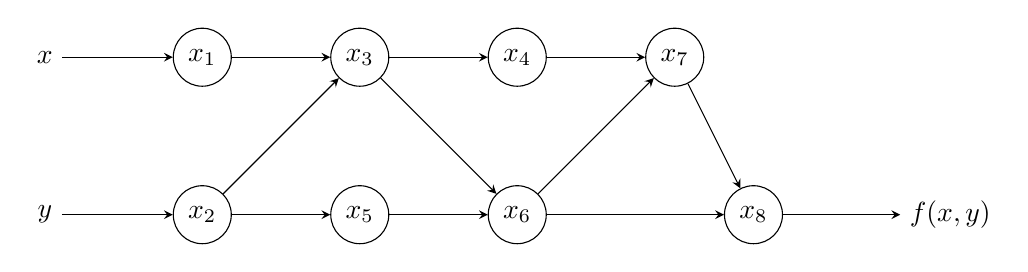
\begin{tikzpicture}
        % Inputs
        \node (y) at (1,2) {$y$};
        \node (x) at (1,4) {$x$};
        
        % Successive nodes
        \node[draw, circle] (x1) at (3,4) {$x_1$};
        \node[draw, circle] (x2) at (3,2) {$x_2$};
        \node[draw, circle] (x3) at (5,4) {$x_3$};
        \node[draw, circle] (x4) at (7,4) {$x_4$};
        \node[draw, circle] (x5) at (5,2) {$x_5$};
        \node[draw, circle] (x6) at (7,2) {$x_6$};
        \node[draw, circle] (x7) at (9,4) {$x_7$};
        \node[draw, circle] (x8) at (10,2) {$x_8$};
        \node (f) at (12.5,2) {$f(x,y)$};
        
        % Edges
        \draw (x) edge[->, >=stealth] (x1)
              (y) edge[->, >=stealth] (x2)
              (x2) edge[->, >=stealth] (x3)
              (x2) edge[->, >=stealth] (x5)
              (x1) edge[->, >=stealth] (x3)
              (x3) edge[->, >=stealth] (x4)
              (x3) edge[->, >=stealth] (x6)
              (x5) edge[->, >=stealth] (x6)
              (x4) edge[->, >=stealth] (x7)
              (x6) edge[->, >=stealth] (x7)
              (x6) edge[->, >=stealth] (x8)
              (x7) edge[->, >=stealth] (x8)
              (x8) edge[->, >=stealth] (f);
    \end{tikzpicture}
    \caption{\textbf{A computational graph.} The function given equation \eqref{eq:ex2} takes two inputs, $x$ and $y$. Standard elementary operations are performed on the inputs to produce a single output, $f(x,y)$.}
    \label{fig:cg-ex2}
\end{figure}
% Computational trace
\begin{table}[H]
    \centering
    \begin{tabular}{lclclcl}
         $x_1$&=&$x$&=&1.5000&&\\
         $x_2$&=&$y$&=&0.5000&&\\
         \hline\hline
         $x_3$&=&$x_1/x_2$&=&1.5000/0.5000&=&3.000\\
         $x_4$&=&$\sin(x_3)$&=&$\sin(3.0000)$&=&0.1411\\
         $x_5$&=&$\exp(x_2)$&=&$\exp(0.5000)$&=&1.6487\\
         $x_6$&=&$x_3-x_5$&=&3.0000-1.6487&=&1.3515\\
         $x_7$&=&$x_4+x_6$&=&0.1411+1.3513&=&1.4924\\
         $x_8$&=&$x_7\times x_6$&=&1.4924$\times$1.3513&=&2.0167\\
         \hline\hline
         $f$&=&$x_8$&=&2.0167&&
    \end{tabular}
    \caption{A typical computational trace using the example given in equation \eqref{eq:ex2}.}
    \label{tab:trace-ex}
\end{table}

\section{Usage Guide}
\subsection{Installation}
Assuming that the user already has the latest version of Python and a package
manager of choice installed, the first step towards using \texttt{AutoDiff} will
be the installation. This can be accomplished using \texttt{conda} or
\texttt{pip}, the two most popular package managers. This process will vary
slightly, depending on the operating system, but essentially, the user will
execute commands from the terminal to update the package manager and install
\texttt{AutoDiff}. 
\begin{minted}{bash}
# Using conda
conda update conda
conda install -c conda-forge AutoDiff

# Using pip
pip install AutoDiff
\end{minted}
\subsection{Getting Started}
Once \texttt{AutoDiff} is installed, the user must import it to be able to use it.
The user will have the option to either import the entire library or to choose
only a subset of modules, classes, or methods to import. For instance, if the user
only wishes to import the automatic differentiation class (and all of its methods)
for linear functions of the form $f(x) = \alpha x + \beta$, then they will have
the freedom to do so. It is widely accepted as good practice to use an alias when
importing libraries. In the following example, the alias for
\texttt{AutoDiff.linear} is just \texttt{linear}. Users will have the ability to
define their own alias.
\begin{minted}{python}
# Imports the necessary constructors and elementary functions 
# (sin, exp, sqrt, etc.) 
from AutoDiff import *

# Only imports forward mode automatic differentiation for linear functions
import AutoDiff.linear as linear
\end{minted}
 

\subsection{Example Usage}
Here we use few simple examples to illustrate the API and data structures of the 
\texttt{AutoDiff} module.
\begin{minted}{python}  
import AutoDiff as ad

# A differentiable object instantiation
x = ad.Variable(3.0)
print(x.val, x.der)
# output: 3.0 0.0

y = x**2
print(y)
# output: AutoDiff(2.25, [3.0])

# What is dy/dx?
print y.der
# output: 3.0

# Specify both the function and derivative values
f = ad.linear(3.0, [2.1])

# Specify the function value only
# The derivative value will default to 1.0 for linear functions.
g = ad.linear(2.0)
\end{minted}

Instances of other classes pertaining to \texttt{AutoDiff} would be 
defined in a similar manner. Once the user defines an instance of a class, they
may perform standard elementary operations on that object. For example,
\texttt{f*g} would return a new object whose function value is the product of the
function values of \texttt{f} and \texttt{g} and whose derivative value is the
product of the corresponding derivative values of \texttt{f} and \texttt{g},
according to the product rule. 
\begin{equation}
    \left.\frac{d}{dx}(fg)\right|_{x=a} 
    = 
    \left.\vphantom{\frac{d}{dx}}f'(x)g(x) + f(x)g'(x)\right|_{x=a}
\end{equation}
This way, the user would have the ability to calculate derivatives of 
composite functions using elementary operations while retaining arbitrary 
precision at each evaluation step. Suppose our expression is $z = x_1 \sin(x_2)$.
\begin{minted}{python} 
import numpy as np
# Multivariate Examples
x1 = ad.Variable(1.0)
x2 = ad.Variable(np.pi/2)
z = x1 * sin(x2)
print(z)
# output: AutoDiff(1.0, array[1.0, 1.0])
# array: dz/dx1, dz/dx2
\end{minted}
As can be seen in the examples, when an \texttt{AutoDiff} object is printed out,
we see two sets of numbers. The first is the current value. The next set of values
are the derivatives of each variable, evaluated at the nominal value.
\section{Software Organization}
\subsection{Directory Structure}
 {\color{blue} /Ccs207-FinalProject}\\
    \hspace*{1cm}{\color{blue}/src}  \hfill Back-end source code\\
		\hspace*{1cm}\hspace*{1cm}{\color{blue}/config} \hfill Configuration for the project\\
		\hspace*{1cm}\hspace*{1cm}{\color{blue}Auto\_diff.py} \\
		\hspace*{1cm}\hspace*{1cm}{\color{blue}forward.py} \\
		\hspace*{1cm}\hspace*{1cm}{\color{blue}reverse.py} \\
		\hspace*{1cm}\hspace*{1cm}{\color{blue}basic\_funcs.py (add by Xin)} \\
		\hspace*{1cm}\hspace*{1cm}{\color{blue}...} \\
	\hspace*{1cm}{\color{blue}/gui}  \hfill Front-end source code \\
		\hspace*{1cm}\hspace*{1cm}{\color{blue}/dist}\hfill Static css, js etc.\\
		\hspace*{1cm}\hspace*{1cm}{\color{blue}/template}\hfill Web html files\\
		\hspace*{1cm}\hspace*{1cm}{\color{blue}/img}\hfill Images used for font-end\\
	\hspace*{1cm}{\color{blue}/utils}  \hfill Preprocessing scripts \\
	\hspace*{1cm}\hspace*{1cm}{\color{blue}input\_parser.py}\\
	\hspace*{1cm}\hspace*{1cm}{\color{blue}...}\\
	\hspace*{1cm}{\color{blue}/test} \hfill Test cases \\
	\hspace*{1cm}\hspace*{1cm}{\color{blue}test\_forward.py}\\
	\hspace*{1cm}\hspace*{1cm}{\color{blue}test\_reverse.py}\\
	\hspace*{1cm}\hspace*{1cm}{\color{blue}test\_eval.py}\\
	\hspace*{1cm}\hspace*{1cm}{\color{blue}...}\\
    \hspace*{1cm}{\color{blue}/doc} \hfill Documentation and records\\
          \hspace*{1cm}\hspace*{1cm}{\color{blue}milestone1.tex}\\
          \hspace*{1cm}\hspace*{1cm}{\color{blue}milestone2.tex}\\
          \hspace*{1cm}\hspace*{1cm}{\color{blue}...}\\
    \hspace*{1cm}{\color{blue}\_\_init\_\_.py} \hfill Initialization\\
    \hspace*{1cm}{\color{blue}requirements.txt}\hfill Packages on which the program depends\\
	\hspace*{1cm}{\color{blue}README.md} \hfill Introduction for the project
\subsection{Modules and functionality}
We plan to include: 
\begin{itemize}
    \item AutoDiff module for definition of the AutoDiff class.
    \item Forward module for forward mode in automatic differentiation.
    \item Reverse module for reverse mode in automatic differentiation.
    \item Some Utils modules for parsing the input, preprocessing and start main program.
\end{itemize}
 
\subsection{Test Suite}
Coding is the fundamental part of software development. Equally significant is build and testing. We would utilize \emph{Travis CI} and \emph{CodeCov} to make the development process more reliable and professional. The test suite will be placed in the test folder.
\begin{itemize}
    \item \emph{Travis CI} is used as a distributed CI (Continuous Integration) tools to build and automate test the project.
    \item \emph{CodeCov} is used for test results analysis (eg. measuring test code coverage) and visualization.
\end{itemize}
 

\subsection{Software Package and Distribution}
\begin{itemize}
    \item  Package distribution\\
    We will package our software using PyPI (Python Package Index) for release. 
    Write and run 'setup.py' to package the software and upload it to the distribution server, thus people in community could easily download our package by 'pip install'.
    \item Version Control\\
    We will take Version Control into consideration according to the standard in Python Enhancement Proposal (PEP) 386. With version control, we can tell the user what changes we made and set clear boundaries for where those changes occurred.
    \item Framework
    \begin{itemize}
        \item For web development, we would use \emph{Flask}, a micro web framework, which is suitable for a small team to complete the implementation of a feature-rich small website and easily add customized functions.
        \item For GUI (Graphical User Interface), we may choose Vue.js, a JavaScript framework for building user interfaces and single-page applications. Because it offers many API (Application Program Interface) to integrate with existing projects and is easy to get started. It is better in code reuse compared to frameworks like jQuery.

    \end{itemize}
    
    
\end{itemize}






\section{Implementation}
\textit{Reverse Mode} and \textit{Forward Mode} will be implemented separately with different data structures but shared basic functions like \mintinline{Python}{Add}, \mintinline{Python}{Mul} in the file \textit{basic\_funcs.py}.

\subsection{Reverse Mode}
\paragraph{Data Structure:}The first step is to parse the input equation into a computational graph for the forward pass. Every leaf variables~(aside from constants) is an instance of \mintinline{Python}{Node}. Computation between leaf variables will be reloaded and return a new node. By doing this, we can parse the input equation into a computational graph automatically. 
\paragraph{Classes and attributes:}Every node in the computation graph is an instance of class \mintinline{Python}{Node} which includes \mintinline{Python}{self.inputs}, the input nodes of current node.
\newline\mintinline{Python}{compute(self, node, input_vals)} and \mintinline{Python}{gradient(self, node, output_grad)}. 
\paragraph{Methods:}Since the order of gradient computing is crucial for \textit{Reverse Mode}, we will use a simple algorithm which does a post-order Depth-First-Search~(DFS) traversal on the given nodes in the computational graph, going backwards based on input edges. With post-order DFS, a node will be added to the ordering after all its predecessors are traversed and we can get a topological sort finally. Then, we can reverse the topological sort list of nodes and start from the output nodes to compute gradient. Pseudo codes are shown as follows,
\begin{minted}{python}
def gradient(out):
    node_to_grad = {}
    nodes = get_reverse_topo_order(out)
    for node in nodes:
        # get gradient of current node
        grad = sum(partial_adjoints from output_edges)  
        # get partial gradient of input nodes of current node
        input_grads = [node.gradient(i, grad) for i in node.inputs]
        add input_grads to node_to_grad
    return node_to_grad
\end{minted}
\paragraph{External dependencies:} Numpy is used to support operations between matrix like \mintinline{python}{MatMul}. 
\paragraph{Elementary Functions:} We will implement them inside the class of \mintinline{Python}{Node}. For example, for the method of \mintinline{Python}{__add__}, we can implement it as follows,
\begin{minted}{python}
class Node(object):
    def __add__(self, other):
        if isinstance(other, Node):
            new_node = add_op(self, other)
        else:
            new_node = add_byconst_op(self, other)
        return new_node
     # Allow left-hand-side add and multiply.
    __radd__ = __add__
\end{minted}

\subsection{Forward Mode}
\textit{Forward Mode} is easier than \textit{Reverse Mode} to implement with different data structure. 
\paragraph{Data Structure:}We will use \mintinline{Python}{STACK} as the main data structure. Basically, each equation can be computed sequentially with Reverse Polish notation~(RPN). For each node, we have to carry derivatives along with evaluation flow. In addition, we have to save the whole graph because we do not know whether we will use them again. 
\paragraph{Classes and attributes:}We will use the class of \mintinline{Python}{Node} again. However, we don't have to maintain the whole graph this time.
Following the order of RPN, a new node will be added with two main attributes, \mintinline{Python}{value} and \mintinline{Python}{derivation}. 

It is worth mentioning that \mintinline{Python}{derivation} of each node is a list with the same length. Specifically, the first element of the list is the derivation of the first leaf variable with respect to the current node. In addition, \mintinline{Python}{derivation} is computed based on the type of gradient and the input gradient. 



\section{Bibliography}
Andreas Griewank. \emph{Evaluating derivatives: principles and techniques of algorithmic differentiation}. 2000.
\end{document}
